Primul procesor superscalar de 32 de biti creat de intel a fost intel Pentium, in 1993, bazat pe
microarhitectura P5. Acesta are 2 pipeline-uri care permit executarea a 2 instructiuni in paralel.

Primul pipeline (U) este pipeline-ul principal, in care se poate executa orice instructiune
citita. Cel de-al doilea pipeline (V) este un pipeline mai simplu, care poate executa majoritatea
instructiunilor, cu putine exceptii\cite{palacharla1997complexity}.

Numarul de stagii in acest pipeline este de 5 \cite{hwu1993superblock}, dar cu fiecare arhitectura nou creata, numarul de
stagii in lungime a crescut, astfel primele procesoare pentium 4 avea un pipeline de 20 de stagii,
comparativ cu cele 10 stagii ale lui pentium 3. Acest lucru a fost necesar pentru a putea marii
frecevnta procesoarelor. Desi mai multe stagii de pipeline inseamna un timp mai mare pentru
executarea unei instructiuni, inseamna si stagii mai simple, cu mai putini tranzistori care pot
rula la frecvente mai mari. Din aceasta motiv in cazul lui pentium 4 Prescott, numarul de stagii a
ajuns la un numar de 31.

\begin{figure*}[ht] \centering
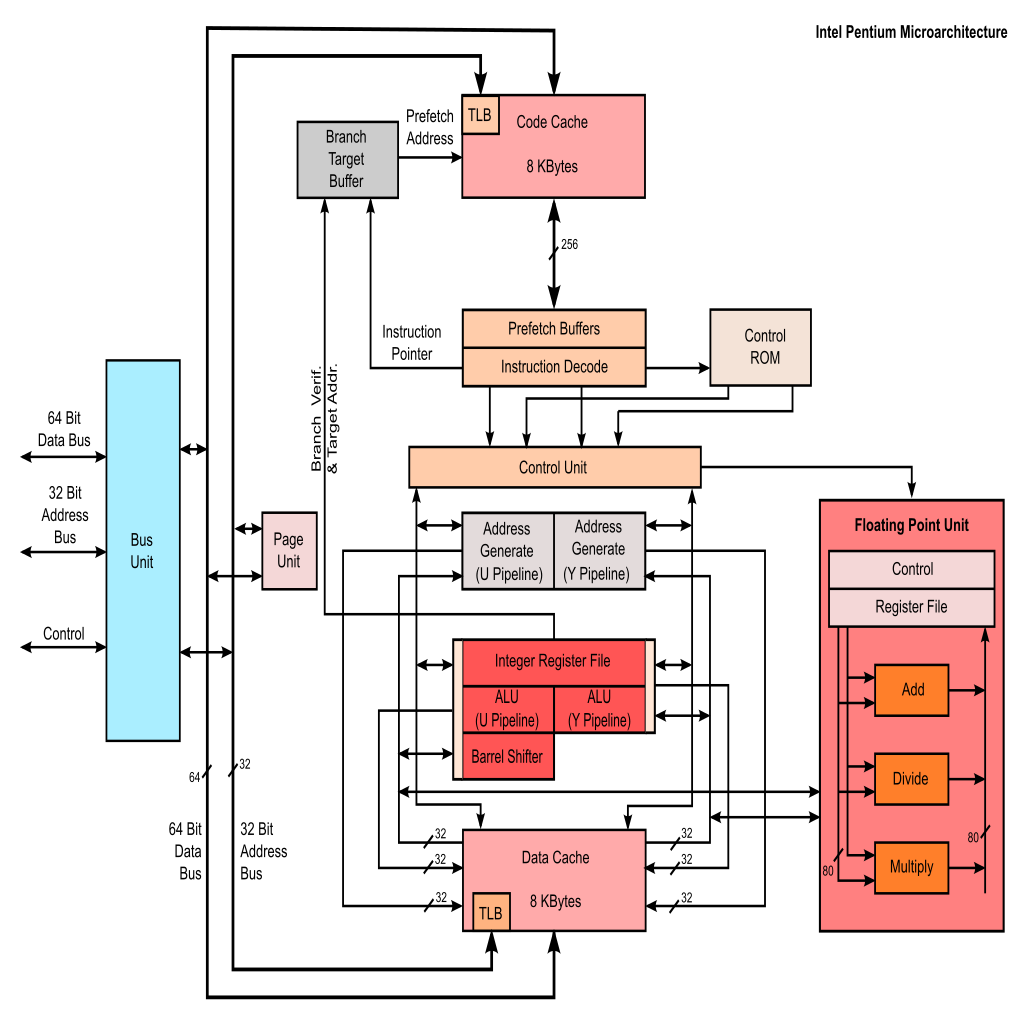
\includegraphics[width=0.6\textwidth]{img/pentiumarch.png}
\caption{Microarhitectura P5} \end{figure*}

\begin{figure*}[ht] \centering

\includegraphics[width=0.9\textwidth]{img/pentium4pipeline.jpg}
\caption{Cele 20 de stagii ale lui pentium 4} \end{figure*}

Generatia urmatoare, microarhitectura core, a micsorat numarul de stagii la 12-14, ceea ce a dus la
reducerea frecventei de lucru, dar pentru a compensa reducerea frecventei s-a dublat latimea pipeline-ului, de la 2 instructiuni executate
in paralel, la 4 instructiuni executate in paralel. Consumul a fost mult miscsorat, scazand de la
130 Watti la 65 de Watti, in principal datorita frecventei reduse, dar performanta acestora este
net superioara, chiar daca functioneaza la frecvente reduse.

Urmatoarea arhitectura, intel Core i7(Nehalem) a marit iar numarul de stagii de pipeline la 20 (
daca operatia de cache a fost de tip hit) sau 24 (daca operatia a fost de tip miss) ca in
generatiile urmatoarea, incepand de la Sandy Bridge, si continuand cu Ivy Bridge si Haswell sa
foloseasca un pipeline cu 14 stagii pentru cache hit si 19 stagii pentru cache miss. Numarul
micsorat de stagii fata de Nehalem au permis o imbunatatire a IPC-ului de pana la 20\%.

\subsection{SMT}

Arhitectura superscalara poate executa doua sau mai multe instructiuni in paralel, dar doar
instructiuni ale aceluiasi program. Din moment ce pipeline-ul a fost paralelizat, urmatorul pas a
fost simularea unui nou nucleu. Acest lucru a fost posibil dubland registrii de baza, pentru a
putea avea 2 program counter si a putea rula instructiuni de la adrese diferite, instructiuni care
nu erau consecutive. Chiar daca sistemul de operare vedea 2 nuclee fizice, in realitate era un
singur nucleu fizic, care putea rula instructiuni de la 2 programe diferite in paralel. Acest lucru
permite folosirea unitatilor procesorului la capacitate maxima.

